%~~~~~~~~~~~~~~~~~~~~~~~~~~~~~~~~~~~~~~~~~~~~~~~~~
% Riichi Book 1, Chapter 2: Tenhou guide 2
%~~~~~~~~~~~~~~~~~~~~~~~~~~~~~~~~~~~~~~~~~~~~~~~~~
\chapter{Advanced features of {\jap Tenhou}} \label{ch:Tenhou2}
\thispagestyle{empty}

\section{Rank and rating}

\begin{floatingtable}[r]{
\footnotesize \captionsetup{font=footnotesize}
\centering 
\begin{tabular}{l r r r}
\toprule
Rank & N & Rank & N\\
\midrule
天鳳位	&9\\
十段	&15&	1級	&7780\\
九段	&130&	2級	&5849\\
八段	&592&	3級	&6481\\
七段	&1830&	4級	&6383\\
六段	&3140&	5級	&6971\\
五段	&5968&	6級	&9964\\
四段	&9957&	7級	&16606\\
三段	&14436&	8級	&14509\\
二段	&18174&	9級	&28283\\
初段	&15046&	~~~新人&132411\\
\bottomrule
\end{tabular}}
\caption{Player distribution} \label{tbl:rank}
\end{floatingtable}

{\jap Tenhou} has two different player rating systems --- rank ({\jap kyu / dan}) and R (rate). 
The {\jap kyu / dan} ranking system is similar to the one commonly used in Japanese arts, games, and martial arts. 
The {\jap kyu} (級) ranks are shown in arabic numbers, going from 9級 to 1級 in descending order. After passing 1級, you enter the {\jap dan} (段) ranks, shown in {\jap kanji} numbers, going from 初段 (一段; first {\jap dan}) to 十段 (tenth {\jap dan}) in ascending order. Everyone starts with {\jap 新人} (newbie; no rank), and if you pass the 十段 rank, you are awarded the highest rank called 天鳳位 ({\jap Tenhoui}). Since the inception of {\jap Tenhou} in 2006, there have been only nine players who have achieved 天鳳位 at the time of writing this book. 
Table \ref{tbl:rank} shows the distribution of active players holding each rank as of 20 December, 2015. 

\bigskip

\subsection{{\jap kyu / dan} rank}

To advance your {\jap kyu / dan} rank, you need to earn points (called ``pt'' or ``段位 pt'' on {\jap Tenhou}). For example, to proceed from the 新人 (newbie) status to the 9 級 ({\jap kyu}) rank, you need to earn 30 points. Required amount of points for promotion gets greater and greater as you move further up. For example, to proceed from 六段 (sixth {\jap dan}) to 七段 (seventh {\jap dan}), you need to earn as many as 1200 points. 

\bigskip
To find out how many more points you need to earn to advance to the next rank from the current rank, see the top right part of the main page. 

\bigskip

\begin{center}
\begin{overpic}[width=.5\textwidth,clip]{figs/rank2.jpg}
\linethickness{2pt}
\put(-5,35){\color{MyRed} \vector(5,-3){50}}
\put(-70,36){\color{MyRed}\small\bf Your current}
\put(-70,16){\color{MyRed}\small\bf rank (7級)}
\put(175,50){\color{MyRed} \vector(-4,-2){85}}
\put(175,50){\color{MyRed}\small\bf pt you have / }
\put(175,30){\color{MyRed}\small\bf pt you need }
\put(110,-13){\color{MyRed} \vector(0,1){15}}
\put(100, -20){\color{MyRed}\small\bf Your R}
\end{overpic}
\vspace{10pt}
\end{center}
\noindent In this example, the player currently holds the rank of 7級. The part that reads ``30 / 60 pt'' means that he has earned 30 points since he became 7級 and that he needs 60 points in total to be promoted to 6級. 

\bigskip
When you rise or fall in rank, your points will be reset to a default value. For {\jap kyu} rank players, the default value is 0 points. For {\jap dan} rank players, the default value is different depending on ranks. For example, the default points for 六段 players are 1200 points. When they get 1200 more points and reach 2400 points, they get promoted to 七段. When they lose all the initial 1200 points and reach 0 points, they get demoted to 五段. 

\bigskip

The amount of points you earn or lose in each game depends on your placement (but \emph{not} scores with {\jap uma} and {\jap oka}), the type of game (East-only or East--South), the room in which the game is played (一般, 上級, 特上, or 鳳凰), and your current rank.\footnote{Points you earn or lose in East-only games are two-thirds of those in East--South games.} 
You gain positive points only if you come in first or second place. 
If you come in first place, you will gain the following points regardless of your rank.

\bi \itemsep-.5em
	\i 45 points in the 一般 ({\jap ippan}) room
	\i 60 points in the 上級 ({\jap joukyu}) room
	\i 75 points in the 特上 ({\jap tokujou}) room
	\i 90 points in the 鳳凰 ({\jap houou}) room
\ei
If you come in second place, you will gain the following points regardless of your rank.
	\bi \itemsep-.5em
	\i 0 points in the 一般 room
	\i 15 points in the 上級 room
	\i 30 points in the 特上 room
	\i 45 points in the 鳳凰 room
\ei
You don't gain or lose points if you come in third place. 
The points you lose when coming in fourth place depend on your rank but not on the room. When your rank is 3級 or below, you lose 0 point. However, each time your rank rises above 3級, the points you lose get bigger by 15 points. 
That is, 2級 players lose 15 points if they come in fourth place; 1級 players lose $15 \times 2 = 30$ points; 初段 players lose $15 \times 3 = 45$ points, ... , and 十段 players lose as many as 180 points if they come in fourth place.

\bigskip
Notice how severe the punishment is for coming in fourth, and it gets severer and severer as your rank goes up. This is one of the distinctive features of {\jap Tenhou}. 
Avoiding the fourth place tends to be players' top priority in {\jap Tenhou} games. This is in contrast to standard mahjong games, where the reward for coming in first usually outweighs the cost of coming in fourth, thanks to the {\jap oka} system.\footnote{Recall that, although {\jap Tenhou} does adopt the {\jap oka} system, it is the placement, not the scores, that determines the points you earn or lose. In this sense, EMA games are actually more similar to {\jap Tenhou} games than to standard games.\index{european@EMA} Since there is no {\jap oka} in EMA games, the reward for coming in first is much smaller than that in standard games.} \index{oka@{\jap oka}}

\bigskip

\begin{wrapfigure}{t}{50mm}
\vspace{-10pt}
\begin{center}
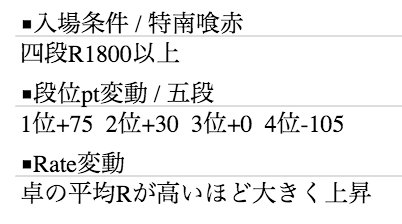
\includegraphics[width=.45\textwidth,clip]{figs/pt}
\end{center}
\vspace{-20pt}
\end{wrapfigure}
To easily find out how many points you earn / lose for each place in a given type of game for your rank, mouseover the \fbox{予約} button in each cell on the left-hand side of the main page. Then, you will see something like the picture above on the right-hand side of the main page. Under the second bullet point, we see that, for this player's rank (五段), the point reward is: +75 for first place, +30 for second place, 0 points for third place, and $-105$ for fourth place. 

\bigskip
\begin{wrapfigure}{r}{60mm}
\vspace{-30pt}
\begin{center}
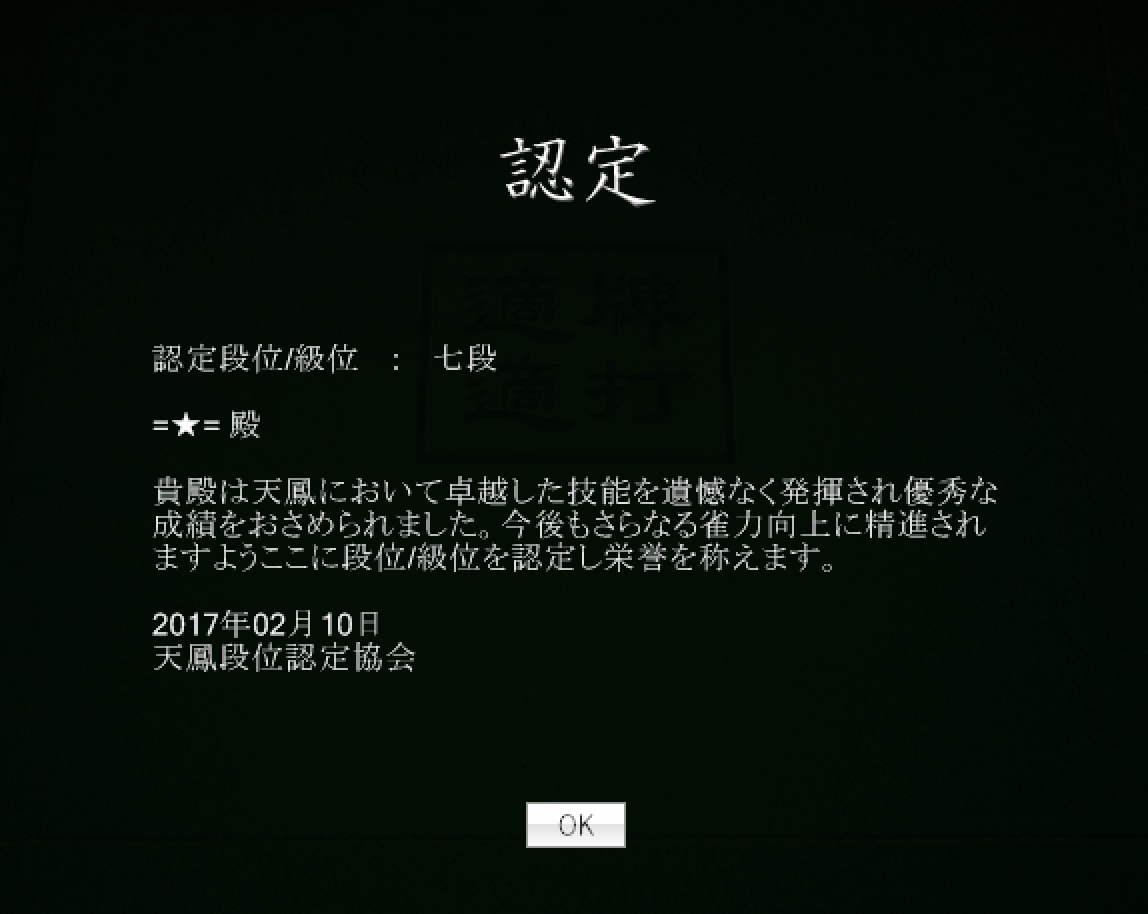
\includegraphics[width=.45\textwidth,clip]{figs/7dan}
\end{center}
\vspace{-25pt}
\end{wrapfigure}
When you earn enough points for promotion in a game, a new rank is awarded after the game. A certificate message like the picture to the right of this text will pop up after the game. 

\bigskip
Since you never get negative points in games until you reach 2級 and there is no demotion until you reach 初段 (first {\jap dan}), it should be relatively easy to reach 初段. In fact, even without studying the contents of this book, you can perhaps reach as high as 四段 (fourth {\jap dan}) if you play a few hundred games or so. However, moving further up will probably require that you study basic strategies and tile efficiency theories. 

\subsection{Rate (R)}

In addition to the {\jap kyu / dan} rank, {\jap Tenhou} gives each player another rating called R. The initial value of R is 1500, and higher-rank players tend to have a higher R. For example, the average R among the 天鳳位 players is 2248.%\footnote{In case you are curious, the highest R I have reached as of December 2015 is 2106.}

\bigskip
While {\jap kyu / dan} rank remains relatively stable, R can change after each game. R is calculated based on your placement in a game, but it also depends on the average R of the players you play with. 
A change in R after a game, $\Delta R$, is calculated with the following formula:
\begin{align*}
\Delta R &= (P + \bar{R}) \times G
\end{align*}
where 
\bi \itemsep-.5em
\i $P$ is based on your placement in the game: + 30 for first, +10 for second, $-$10 for third, and $-$30 for fourth;
\i $\bar{R}$ is an adjustment that reflects how strong your opponents are, calculated as (Average R in the game $-$ your R) $/$ 40; and
\i $G$ is an adjustment based on $n$, the number of games you have played before. If $n \leq 400$, G is equal to $1-0.002 \times n$. If $n > 400$, G is set equal to 0.2.
\ei

\bigskip
R initially fluctuates a lot, as the scaling factor $G$ is very close to 1 until you play many games. R may go up or down by 30 or so for each of the first 100 games or so. As you play more games, however, the fluctuation gets smaller and smaller as $G$ approaches to $0.2$. 

\bigskip
Notice what the adjustment $\bar{R}$ does. This factor is positive when you play against players who are ``stronger'' than you (i.e., have a higher R than you) while it is negative when you play against players who are ``weaker'' than you. Therefore, when you win against stronger players, your reward will be bigger than when winning against weaker players. Likewise, when you lose against weaker players, your punishment will be severer than when losing against stronger players. 
Because of these features, one might say that your R better reflects your skill levels than your {\jap kyu / dan} rank. 

\section{Four rooms}
As we have seen, there are four different rooms where ranking matches are played. Qualifications to play in each room are based on your rank and R. 

\subsection*{1. 一般 ({\jap ippan}; lower-level room)}
This is the only room where you can play initially. Players with an R higher than 1800 and a rank higher than 四段 are not allowed to play here, however. Games in this room can sometimes be a bit random, even chaotic at times. Some of the players in this room probably do not understand the rules very well. You very rarely come across strong players here. 

\subsection*{2. 上級 ({\jap joukyu}; upper-level room)}
You can play here if (1) your rank is 1級 or higher or (2) you buy a two-month membership (\textyen~1080 = \euro~8 = \textsterling~6).\footnote{If you want to pay for the membership, click on the link that appears when you click the 上級 sub-tab. Keep in mind that you need to buy 60 days' worth of membership. Choose ``60日分を購入(1080円)'' in the payment page.} Players with an R higher than 2000 and a rank higher than 七段 are not allowed to play in this room, however. 

\bigskip
Games in the {\jap joukyu} room are more reasonable than those in the lower-level room, but you still see many players who do not defend at all, do meaningless {\jap dama} / unreasonable riichi, and make serious mistakes in maximizing tile efficiency. In my impression, games at EMA tournaments most resemble games in the {\jap ippan} and {\jap joukyu} rooms.\index{european@EMA} 

\subsection*{3. 特上 ({\jap tokujou}; advanced room)}
Requirements to play in this room are pretty demanding. You have to have a 四段 or higher rank and a 1800 or higher R. The latter requirement is particularly difficult to satisfy for intermediate players. As I wrote above, achieving the rank of 四段 is not that difficult, but satisfying the R $\geq$ 1800 condition requires that you take mahjong rather seriously. Since weak players are shut out from the {\jap tokujou} room, games in {\jap tokujou} are qualitatively different from those in the {\jap joukyu} and {\jap ippan} rooms. Games in this room feel similar to those you'd experience at regular フリー ({\jap furii}) mahjong parlors in Japan. 

\subsection*{4. 鳳凰 ({\jap houou}; phoenix room)}
This is the highest-level room in {\jap Tenhou}. In order to play in this room, you have to have all of the following: (1) a 七段 or higher rank, (2) a 2000 or higher R, and (3) a paid membership (\textyen~540 yen = \euro~4 = \textsterling~3 per month). Satisfying the first two conditions can be really, really challenging. 

\bigskip
This is arguably one of the highest-level mahjong locales in the whole world. It is not uncommon for you to come across a {\jap houou}-level player at a regular mahjong parlor in Japan. However, you usually play against at most one {\jap houou}-level player at a table, and the two other players at the table are either {\jap tokujou}- or {\jap joukyu}-level players. What is remarkable about games in the {\jap houou} room is that you will be surrounded by three other {\jap houou}-level players. 
It would be safe to say that no other public mahjong locale in the world --- whether it is online or offline --- could offer a comparable experience.\footnote{Perhaps the highest-level leagues in professional mahjong associations in Japan have players who are of comparable quality, but you have to become a professional player to play at such leagues. Even after becoming a professional, you will need at least a few years to reach the highest league.}

\section{Reading the statistics}
After you play 30 games or so, you may want to start paying attention to the statistics shown on the right-hand side of the main page.\footnote{There is really no point in reading too much into the statistics when you have played only a few games; the sample size is too small to be meaningful.} 
The upper half of the player statistics shows your statistics for the entire period, whereas the bottom half shows your statistics in the present month for a given type of game in a given room. 

\bigskip
\subsection{Overall statistics}
The picture below show my old player statistics (upper half) back from when I had a 二段 rank. 
Let me explain how to read these statistics. 

\begin{center}
\vspace{-10pt}
\begin{overpic}[width=.6\textwidth,clip]{figs/stats1_anon.jpg}
\linethickness{2pt}
\put(-52,92){\color{MyRed}\small Entire period}
\put(133,92){\color{MyRed}\small (4-player games)}
\put(-60,62){\color{MyRed}\small first place}
\put(-60,49){\color{MyRed}\small second place}
\put(-60,36){\color{MyRed}\small third place}
\put(-60,23){\color{MyRed}\small fourth place}
\put(-60,10){\color{MyRed}\small bankruptcy}
\put(200,60){\color{MyRed}\small win rate}
\put(200,47){\color{MyRed}\small deal-in rate}
\put(200,34){\color{MyRed}\small call rate}
\put(200,21){\color{MyRed}\small riichi rate}
\end{overpic}
\vspace{-10pt}
\end{center}

Below a player name is the expiration date of my premium membership (17 November, 2015). When I started playing {\jap Tenhou} on 17 September, 2015, I bought a 60-day membership so I can play in the {\jap joukyu} room. If you have just created a {\jap Tenhou} account, the expiration date will be shown as today's or tomorrow's date, since we are given a 1-day premium membership when we open an account.\footnote{You need to have a premium membership to use {\jap Tenhou}'s Windows client.} After a day or two, it will turn into ``----/--/--'' meaning that you do not have a premium membership.

\bigskip

The box below the expiration date that reads 全期間 / 段位戦 4人打ち indicates that the statistics below are for the entire period (not just this month) and for 4-player games (not 3-player games). Below that, we see that I had a 二段 rank, 565 points (the initial 400 points plus 165 points earned after I became 二段) out of the 800 points I need for promotion, and an R of 1987. 

\bigskip

Three columns below these display my statistics. The first column shows my placement rates. I had come in first place 50\% of the games, second place 32.5\%, third place 7.5\%, fourth place 10 \%, and gone bankrupt 7.5\% of the games. Ideally, you'd want your first place rate to be greater than your second place rate, your second place rate greater than your third place rate, etc. 

\bigskip

The middle column provides the following information. First, 対戦数 shows the number of games you have played. At this point, I had played 40 games. Second, 平均得点 shows the average score (with {\jap oka} and {\jap uma}) from all the games I have played. As I said before, this does not influence your R nor rank. Third, 平均順位 shows the average placement. If you have obtained each of the four places equally, the average placement would be 2.5 $\left( \frac{1  n + 2  n + 3  n + 4 n}{4n} = 2.5 \right)$. Therefore, any values below 2.5 indicate that you are, on average, winning more than losing. 
The two rows that follow (shown in light gray) are relevant only if you play games in private rooms. Since I have only played ranking matches, they are left blank. 

\bigskip

The third column shows my statistics based on hand-level performance. First, 和了率 ({\jap houra} rate; {\jap agari} rate; win rate) is the number of hands you have won divided by the total number of hands you have played in all games.\footnote{The denominator includes hands where no one won.} 

\bigskip
Second, 放銃率 ({\jap houju} rate; deal-in rate) is the number of times you have fed the winning tile to an opponent's hand divided by the total number of hands you have played. You would want this rate to be lower, but keep in mind that (1) sometimes you would be better off dealing into an opponent's hand to secure your placement, and (2) sometimes you need to discard dangerous tiles (which would increase your deal-in rate, on average) in order to increase the chance of winning your hand (which would increase your win rate, on average). The rule-of-thumb is that the difference between your win rate and deal-in rate (win rate - deal-in rate) should be at least 10 percentage points. That is, if you have a high deal-in rate, you need your win rate to be higher. Likewise, if you have a low deal-in rate, it is OK to have a lower win rate as well. 

\bigskip
Third, 副露率 ({\jap fuuro} rate; call rate) is the number of hands where you have called {\jap chii} / {\jap pon} / {\jap kan} divided by the total number of hands you have played. Finally, 立直率 (riichi rate) is the number of riichi calls you made divided by the number of hands you have played. 

\bigskip

The ranking page on {\jap Tenhou}\footnote{\url{http://goo.gl/suyQ5}} has a table that summarizes the average values of these statistics among players with different ranks (under the heading that reads 段位戦4人打ち平均戦績). You may want to compare your statistics with the average values among players who share your rank or those who have higher ranks than you do. Figure \ref{fig:avg} summarizes the average values of hand-level performance statistics for players in different ranks. 

\begin{figure}[t!] \captionsetup{font=small}
\begin{center}
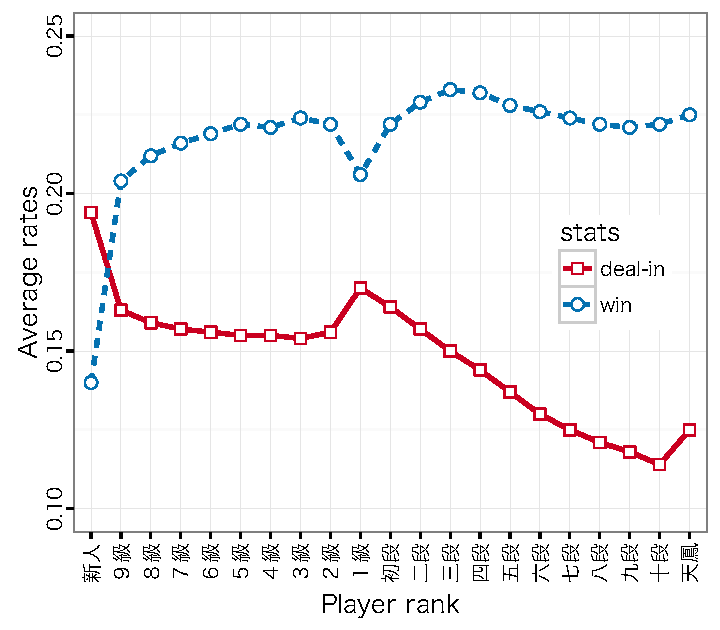
\includegraphics[width=.50\textwidth,clip]{figs/stats_wd.pdf}\hspace{-7pt}
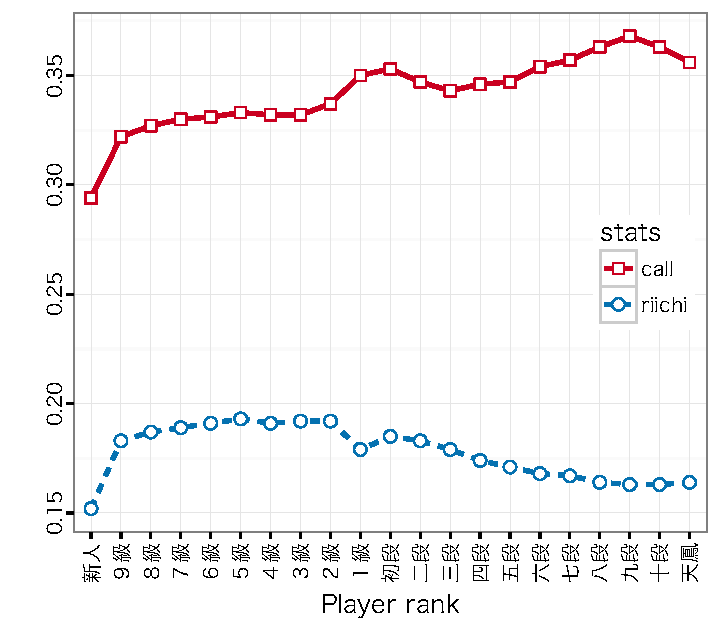
\includegraphics[width=.50\textwidth,clip]{figs/stats_cr.pdf}
\vspace{-10pt}
\caption{Average hand-performance statistics}\label{fig:avg}
\end{center}\vspace{-10pt}
{\footnotesize \textit{Note:} These graphs show the hand-performance statistics reported in a table on the ranking page (\url{http://goo.gl/suyQ5}) as of 20 December, 2015.}
\end{figure}

\bigskip
We can see some interesting patterns here. The left-hand side panel compares average win rates (和了率) and deal-in rates (放銃率) for different ranks. Notice that the average win rate is relatively constant across different ranks; once you pass the 新人 rank, it stays around 20-22 \%. 

\bigskip
On the other hand, the average deal-in rate is steadily decreasing after players move from the {\jap kyu} ranks into the {\jap dan} ranks. It is around 15\% for almost all {\jap kyu} rank players (except for 新人 and 1級), but it keeps going lower and lower as players rise in the {\jap dan} rank. The fact that high-{\jap dan} players have lower deal-in rates on average is remarkable, considering that they are facing stronger opponents than low-{\jap dan} players do. This pattern signifies the importance of defensive skills.

\bigskip

Another interesting thing to notice on the left-hand side panel is that the average scores deteriorate once you move from 2級 to 1級 (i.e., average win rate gets lower, and average deal-in rate gets higher). 

\bigskip
I can think of two reasons for why this happens. First, 1級 is where most players start playing in the {\jap joukyu} (upper-level) room, where average player skills are much higher than those in the {\jap ippan} (lower-level) room. If a player who belongs to the lower-level room plays in the upper-level room, their performance will necessarily go down, making it look that 1級 players are worse than 2級 players even if they are not. Second, if you keep losing as a 初段 (first {\jap dan}) player, you get demoted to 1級 but you will never be demoted to 2級. This means that 1級 players might actually be worse than 2級 players, on average. 

\bigskip

The right-hand side panel shows the average call rates (副露率) and riichi rates (立直率) for different ranks. The former is increasing as rank goes up, while the latter is decreasing, but the changes are rather gradual for both rates. 

\vfill

\subsection{Monthly statistics}
The bottom-right part of the main page shows monthly statistics from games you have played in a given room. The box is a pull-down menu that lets you choose the room (一般, 上級, 特上, 鳳凰) and game type (East-only, East--South, with or without open {\jap tanyao}, red fives, etc.). In the example below, the box reads 月間 / 上南 喰アリ赤, which means the following: 月間 means monthly, 上 is short for 上級 ({\jap joukyu})\footnote{Likewise, 般 is short for 一般 ({\jap ippan}), 特 is for 特上 ({\jap tokujou}), 鳳 is for 鳳凰 ({\jap houou}).}, 喰アリ赤 means with open {\jap tanyao} and red fives.

\begin{center}
%\vspace{-10pt}
\begin{overpic}[width=.6\textwidth,clip]{figs/stats2.jpg}
\linethickness{2pt}
\put(-12,98){\color{MyRed}\small Cumulative}
\put(150,98){\color{MyRed}\small Average}
\put(-23,87){\color{MyRed}\small Scores}
\put(-44,75){\color{MyRed}\small Placement}
\put(-45,26){\color{MyRed}\small first place}
\put(-45,11){\color{MyRed}\small fourth place}
\end{overpic}
\vspace{-10pt}
\end{center}


Below the box, you see the raw placement scores. In this example, 17+11+3+4 = 35戦 means that I have played 35 games this month, and I came in first place in 17 games, second place in 11 games, third place in 3 games, and fourth place in 4 games. R shown here (1987) should be the same as the R you see in the top part. 3382位 means that R=1987 puts me in 3382th place among all the active players on {\jap Tenhou}. 

\bigskip
Two columns follow, where the left column shows the monthly cumulative values and the right column shows the monthly average values. 
In the first row that reads 得点 shows the monthly cumulative or average scores from 上南 喰アリ赤 games (after adding {\jap oka} and {\jap uma}). In this example, my cumulative score is 727 from the 35 games I played, which puts me in 106th place among players who have played 30 or more 上南 喰アリ赤 games this month. Similarly, my average score is 20.7 (= 727/35), which puts me in 5th place. Your placement for average scores will not be shown unless you have played 30 or more games of a given type in a given room in a given month. 

\bigskip
In the second row that reads 順位 shows cumulative or average placement from games. The cumulative placement is based on placement values (+30, +10, $-$10, or $-$30), whereas the average placement is based on raw placement (1, 2, 3, or 4). 
The 総合 (total) score is the sum of four placements: cumulative 得点, cumulative 順位, average 得点, and average 順位. In this example, I earn 106th, 80th, 5th, and 3th places for these scores, so my total score is 106+80+5+3 = 194 (the lower, the better), which puts me in 12th place among all the players who have played 30 or more 上南 喰アリ赤 games this month. 
At the bottom, you see トップ率 (first place rate),  ラス率 (fourth place rate), and 連対率 (first or second place rate) for 上南 喰アリ赤 games this month. 

\section{Viewing games}
\subsection{Game replay (牌譜)}
{\jap Tenhou} keeps the record of all the games played there, giving each game a unique URL. 
You can easily take a look at any of the last 40 games you have played on the 牌譜 ({\jap haifu}; game record) tab on the main page. Click on any of the 牌譜 link shown in the 牌譜 tab to start a replay of the game. You can choose to view the game from any of the four players' viewpoint, not to show the hands of the other three players, or to go back and forth between turns / hands, etc. When we play mahjong, we often wonder what the opponents are doing (e.g., what are their waits? are they doing {\jap honitsu}?, etc.). You can find out the answers to these questions after the game by taking a look at the game record. 

%\bigskip

%\begin{wrapfigure}{r}{60mm}
\begin{center}
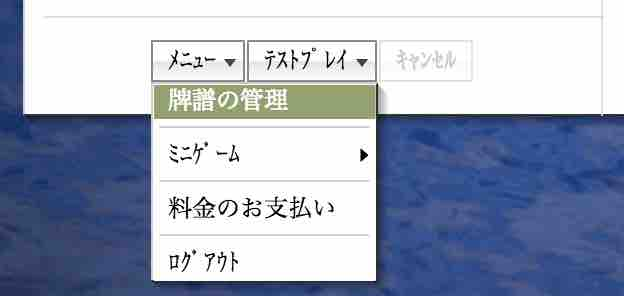
\includegraphics[width=.4\textwidth,clip]{figs/haifukanri.jpg}
\end{center}
%\vspace{-20pt}
%\end{wrapfigure}

If you would like to have someone take a look at a particular game you played to ask for their opinions, you need to find the unique URL assigned to the game you want to show. You can find out the URLs of the last 40 games by going to the 牌譜の管理 menu from the メニュー pull-down on the main page. 
Clicking on 牌譜の管理 will open a new pop-up screen.

\bigskip
You can choose to open a game replay in the current window (このウィンドウで開く), in a new pop-up window (新しいポップアップで開く), or in a new window (新しいウィンドウで開く) from the pull-down menu above. Once you are happy with your choice, click on one of the 再生 (replay) link next to the game you want replayed. 
You will be taken to a page that looks like the one you saw after clicking on the Play button on the top page of {\jap Tenhou}. You can now find out the URL assigned to the game in the URL field of your browser. 

\bigskip
To start a replay, click on a link that reads >> Flash版牌譜ビューアで開く shown at the bottom of the page. Clicking on the HTML+JS版牌譜ビューアで開く link will also work, but this one is the low-quality picture version with limited options. 

\subsection{Spectating games (観戦)}
You can watch games played in the 特上 ({\jap tokujou}; advanced) and the 鳳凰 ({\jap houou}; phoenix) rooms quasi-real time (with a five-minute delay). Click on the 観戦 ({\jap kansen}; spectating) tab from the main page and you will see the list of games you can watch. Click on one of the player name links to start spectating the game from the chosen player's viewpoint. 

